
\section{\trMinimax{}思想}
\label{sec:minimax}

我们考察一个可微函数
\[
f:E\to\R,\qquad f\in C^{1}(E,\R),
\]
它定义在一个\trHilbert{}空间 $E$ 上，其\trInnerProduct{}记作 $\langle\cdot,\cdot\rangle$，%
\trNorm{}为 $\|x\|^{2}=\langle x,x\rangle$（$x\in E$）。我们寻找 $f$ 的诸\trCriticalPoint，%
亦即 $f$ 的\trDerivative{}在其中为零的点 $x^{*}\in E$：
\[
df(x^{*})=0\quad\Longleftrightarrow\quad df(x^{*})(y)=0\quad\text{对一切}\ y\in E.
\]
按定义，$df(x)$ 是\trDual{}空间 $\mathcal{L}(E,\R)=E^{*}$ 的一个元素。%
回顾一下 F.~\trRiesz{}的一个众所周知的定理：存在一个从 $E^{*}$ 到 $E$ 的典范%
\textbf{\trLinear\trIsometry\trIsomorphism}（linear isometry）$I$，使得对每个 $x\in E$ 都有%
$e^{*}(x)=\langle I(e^{*}),x\rangle$，其中 $e^{*}\in E^{*}$。于是，
\[
df(x)(y)=\langle v(x),y\rangle\qquad\text{且}\qquad\|df(x)\|_{*}=\|v(x)\|,
\]
其中 $v(x)\in E$ 由 $df(x)$ 唯一确定。它称为 $f$ 在点 $x$ 处的\trGradient{}%
（相对于\trInnerProduct{} $\langle\cdot,\cdot\rangle$ 而取），并记作
\[
v(x)=\nabla f(x)\in E.
\]

$f$ 的诸\trCriticalPoint{}便是 $E$ 中\trGradient{}函数 $x\mapsto\nabla f(x)$ 的零点。%
借助动力学的观点，我们把 $f$ 的诸\trCriticalPoint{}解释为\trGradient{}方程
\[
\dot{x}=-\nabla f(x),\qquad x\in E
\]
的诸\trEquilibrium。这是 $E$ 上的一个常\trDifferentialEquation，现在我们假定它具有%
整体\trFlow{} $\varphi^{t}(x)$，也就是说，我们可以唯一地、并且对一切时刻 $t\in\R$%
求解\trCauchy\trInitialValueProblem：
\begin{align*}
\frac{d}{dt}\,\varphi^{t}(x)\ &=\ -\nabla f\bigl(\varphi^{t}(x)\bigr)\\
\varphi^{0}(x)\ &=\ x,
\end{align*}
其中 $x\in E$ 为任意初始条件。这样的整体\trFlow{}确实是存在的，譬如，只要存在常数%
$M\geq0$ 使得对一切 $x$, $y\in E$ 都有 $\|\nabla f(x)-\nabla f(y)\|\leq M\|x-y\|$，%
如众所周知的那样。\textbf{\trGradient\trFlow}（gradient flow）的关键性质是：%
$f\bigl(\varphi^{t}(x)\bigr)$ 沿非常值解 $\varphi^{t}(x)$ 递减。这由定义立即可得；事实上
\begin{align*}
\frac{d}{ds}\,f\bigl(\varphi^{s}(x)\bigr)\ &=\ df\bigl(\varphi^{s}(x)\bigr)\Bigl(\frac{d}{ds}\,\varphi^{s}(x)\Bigr)\\
&=\ df\bigl(\varphi^{s}(x)\bigr)\bigl(-\nabla f\bigl(\varphi^{s}(x)\bigr)\bigr)\\
&=\ -\bigl\langle\nabla f\bigl(\varphi^{s}(x)\bigr),\nabla f\bigl(\varphi^{s}(x)\bigr)\bigr\rangle\ .
\end{align*}
特别地，
\begin{equation}\label{eq:gradient-flow-decrease}
f\bigl(\varphi^{t}(x)\bigr)-f(x)\ =\ \int_{0}^{t}\frac{d}{ds}\,f\bigl(\varphi^{s}(x)\bigr)\,ds\ =\ -\int_{0}^{t}\bigl\|\nabla f\bigl(\varphi^{s}(x)\bigr)\bigr\|^{2}\,ds.
\end{equation}
由于 $E$ 不是\trCompact{}的，若不对 $f$ 附加额外的条件，我们便不能指望 $f$ 拥有%
任何\trCriticalPoint，正如 $x\in\R$ 上的函数 $f(x)=e^{-x}$ 这个例子已经表明的那样。%
下述强\trCompactness{}条件可追溯到 \trPalais{}与 \trSmale{} [175]，它在许多\trVariational{}问题中%
保证了\trCriticalPoint{}的存在。

\begin{definition}\label{def:palais-smale}
称 $f$ 满足 P.S.（\trPalaisSmale{}条件），如果每一个满足
\[
\nabla f(x_{j})\rightarrow0\ \text{在}\ E\ \text{中}\qquad\text{且}\qquad\bigl|f(x_{j})\bigr|\leq c<\infty
\]
（对某个 $c\geq0$）的序列 $x_{j}\in E$ 都拥有一个\trConverge{}子序列。由于假定%
$f\in C^{1}$，该子序列的极限便是 $f$ 的一个\trCriticalPoint。
\end{definition}

若 $\mathcal{F}$ 是由子集 $F\subset E$ 组成的一个族，我们如下定义属于 $f$ 与%
$\mathcal{F}$ 的\trMinimax{} $c(f,\mathcal{F})$：
\[
c(f,\mathcal{F})=\inf_{F\in\mathcal{F}}\ \sup_{x\in F}\ f(x)\qquad\in\ \ \R\cup\{\infty\}\cup\{-\infty\}
\]

\textbf{\trMinimax{}引理。}\quad 设 $f\in C^{1}(E,\R)$ 与 $\mathcal{F}$ 满足下列条件：
\begin{enumerate}[label=(\roman*)]
\item $f$ 满足 P.S.；
\item $\dot{x}=-\nabla f(x)$ 定义了一个整体\trFlow{} $\varphi^{t}(x)$；
\item 族 $\mathcal{F}$ 在该\trFlow{}下是正\trInvariant{}的，即若 $F\in\mathcal{F}$，%
则对每个 $t\geq0$ 都有 $\varphi^{t}(F)\in\mathcal{F}$；
\item $-\infty<c(f,\mathcal{F})<\infty$.
\end{enumerate}
那么，实数 $c(f,\mathcal{F})$ 便是 $f$ 的一个\textbf{\trCriticalValue}%
（critical value），也就是说，存在 $x^{*}\in E$ 满足
\[
\nabla f(x^{*})=0\qquad\text{且}\qquad f(x^{*})=c(f,\mathcal{F}).
\]

\begin{proof}
记 $c=c(f,\mathcal{F})$，由假设它是一个实数。我们将证明：对每个 $\varepsilon>0$，%
存在 $x\in E$ 满足
\[
c-\varepsilon\leq f(x)\leq c+\varepsilon\qquad\text{且}\qquad\|\nabla f(x)\|\leq\varepsilon.
\]
然后取 $\varepsilon_{j}=1/j$，便得到一列 $x_{j}$，由 P.S. 条件，它拥有一个%
\trConverge{}子序列，其极限满足 $\nabla f(x^{*})=0$ 与 $f(x^{*})=c$，从而引理得证。%
用反证法，我们找到 $\varepsilon>0$ 使得
\begin{equation}\label{eq:gradient-bound-epsilon}
\|\nabla f(x)\|>\varepsilon
\end{equation}
对一切满足 $c-\varepsilon\leq f(x)\leq c+\varepsilon$ 的 $x$ 成立。由 $c$ 的定义，%
存在 $F\in\mathcal{F}$ 满足
\begin{equation}\label{eq:sup-f-estimate}
\sup_{x\in F}\,f(x)\ \leq\ c+\varepsilon.
\end{equation}
取一点 $x\in F$，则 $f(x)\leq c+\varepsilon$；我们断言，若 $t^{*}=2/\varepsilon$，%
则解 $\varphi^{t}(x)$ 满足 $f\bigl(\varphi^{t^{*}}(x)\bigr)\leq c-\varepsilon$。%
的确，若对某个 $0\leq t\leq t^{*}$ 有 $f\bigl(\varphi^{t}(x)\bigr)\leq c-\varepsilon$，%
则由于 $f\bigl(\varphi^{t}(x)\bigr)$ 是递减的，已无须再证什么。现用反证法假设对一切%
$0\leq t\leq t^{*}$ 都有 $f\bigl(\varphi^{t}(x)\bigr)>c-\varepsilon$。那么由%
\eqref{eq:gradient-bound-epsilon}，对 $0\leq t\leq t^{*}$ 有%
$\|\nabla f\bigl(\varphi^{t}(x)\bigr)\|\geq\varepsilon$，从而由%
\eqref{eq:gradient-flow-decrease} 得 $f\bigl(\varphi^{t}(x)\bigr)\leq f(x)-\varepsilon^{2}t$，%
于是 $f\bigl(\varphi^{t^{*}}(x)\bigr)\leq c+\varepsilon-\varepsilon^{2}t^{*}=c-\varepsilon$，%
矛盾。令 $F^{*}=\varphi^{t^{*}}(F)$，我们便证明了
\[
\sup_{x\in F^{*}}\,f(x)\ \leq\ c-\varepsilon\ .
\]
而由假设 $F^{*}\in\mathcal{F}$，这一\trEstimate{}便与 $c$ 的定义相矛盾。
\end{proof}

\noindent\begin{minipage}{\linewidth}
\centering
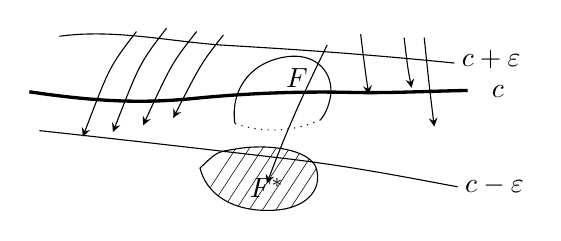
\begin{tikzpicture}[>=stealth,scale=0.85]
  \draw (0,1.85) .. controls (0.8,1.96) and (1.6,1.78) .. (2.4,1.72)
        .. controls (3.4,1.66) and (4.4,1.6) .. (5.9,1.45);%
  \draw[very thick] (-0.45,1.02) .. controls (0.5,0.88) and (1.2,0.84) .. (2.0,0.92)
        .. controls (2.8,1.0) and (3.6,1.03) .. (4.4,1.01)
        .. controls (5.0,1.0) and (5.5,1.03) .. (6.1,1.04);%
  \draw (-0.3,0.44) .. controls (1.0,0.3) and (2.2,0.16) .. (3.4,0.02)
        .. controls (4.4,-0.1) and (5.2,-0.26) .. (5.95,-0.4);%
  \node at (6.45,1.5) {$c+\varepsilon$};
  \node at (6.55,1.02) {$c$};
  \node at (6.5,-0.38) {$c-\varepsilon$};
  \draw[->] (1.15,1.92) .. controls (0.75,1.4) .. (0.35,0.35);
  \draw[->] (1.6,1.97) .. controls (1.2,1.45) .. (0.8,0.42);
  \draw[->] (2.05,1.92) .. controls (1.68,1.45) .. (1.25,0.52);
  \draw[->] (2.45,1.87) .. controls (2.12,1.45) .. (1.7,0.63);
  \draw[->] (4.5,1.88) .. controls (4.56,1.4) .. (4.62,0.98);
  \draw[->] (5.15,1.83) .. controls (5.2,1.4) .. (5.26,1.08);
  \draw[->] (5.45,1.83) .. controls (5.52,1.15) .. (5.6,0.5);
  \draw[->] (4.0,1.72) .. controls (3.75,1.2) and (3.45,0.6) .. (3.1,-0.35);
  \draw (2.62,0.55) .. controls (2.55,1.1) and (2.9,1.5) .. (3.45,1.55)
        .. controls (3.85,1.58) and (4.1,1.3) .. (4.05,0.95)
        .. controls (4.02,0.8) and (3.98,0.7) .. (3.9,0.6);
  \draw[dotted] (3.9,0.6) .. controls (3.5,0.42) and (3.0,0.4) .. (2.62,0.55);
  \node at (3.55,1.22) {$F$};
  \begin{scope}
    \clip (2.1,-0.12) .. controls (2.2,-0.52) and (2.6,-0.78) .. (3.2,-0.75)
          .. controls (3.75,-0.72) and (3.95,-0.38) .. (3.82,-0.08)
          .. controls (3.65,0.2) and (3.0,0.24) .. (2.6,0.16)
          .. controls (2.35,0.12) .. (2.1,-0.12) -- cycle;
    \foreach \d in {1.9,2.1,...,3.9}
      \draw[very thin] (\d,-0.95) -- (\d+0.85,0.35);
  \end{scope}
  \draw (2.1,-0.12) .. controls (2.2,-0.52) and (2.6,-0.78) .. (3.2,-0.75)
        .. controls (3.75,-0.72) and (3.95,-0.38) .. (3.82,-0.08)
        .. controls (3.65,0.2) and (3.0,0.24) .. (2.6,0.16)
        .. controls (2.35,0.12) .. (2.1,-0.12) -- cycle;
  \node at (3.1,-0.42) {$F^{*}$};
\end{tikzpicture}

图 3.5
\end{minipage}

譬如，若 $f$ 还是\trBoundedBelow{}的，我们便可取 $\mathcal{F}$ 为由 $E$ 的元素所组成的%
诸单点集 $\{x\}$ 之族，于是
\[
c(f,\mathcal{F})=\inf_{x\in E}\,f(x).
\]
引理这时便保证了一个最小值，也就是说，我们找到 $x^{*}\in E$ 满足%
$\nabla f(x^{*})=0$ 以及
\[
f(x^{*})=\inf_{x\in E}\,f(x).
\]

作为另一个说明，我们来描述著名的\trMountainPassLemma，它由 A.~\trAmbrosetti{}与%
P.~\trRabinowitz{} [6] 所发现。我们复述的是 R.~\trPalais{}与 C.~\trTerng{}在 [174] 中%
给出的那个颇具观感之美的版本。设 $R\subset E$ 为一子集，若它\trSeparate{} $E$，若
\[
\alpha:=\inf_{R}\,f>-\infty
\]
且在 $E\backslash R$ 的每个\textbf{\trConnectedComponent}（connected component）上，函数 $f$ 都%
取到严格小于 $\alpha$ 的值，则称 $R$ 为相对于 $f$ 的一个\textbf{山脉}%
（mountain range）。考虑一个满足 P.S. 条件的 $f\in C^{1}(E,\R)$，并假定%
\trGradient{}方程生成一个整体\trFlow。

\textbf{\trMountainPassLemma。}\quad 若 $R\subset E$ 是相对于 $f$ 的一个山脉，则 $f$ 拥有一个满足
\[
c\geq\inf_{R}\,f
\]
的\trCriticalValue{} $c$。

\begin{proof}
我们选取 $E\backslash R$ 的两个互不相同的\trConnectedComponent{} $E^{0}$ 与 $E^{1}$，并对%
$j=0,1$ 定义 $E^{j}_{\alpha}=\bigl\{\,x\in E^{j}\ \bigm|\ f(x)<\alpha\,\bigr\}$。%
由假设，这些集合都非空。令 $\Gamma$ 为一切满足 $\gamma(0)\in E^{0}_{\alpha}$、%
$\gamma(1)\in E^{1}_{\alpha}$ 的\textbf{连续\trPath}（continuous path）$\gamma:[0,1]\to E$ 全体，并如下定义由%
$E$ 的\trCompact{}子集所组成的族 $\mathcal{F}$：
\[
\mathcal{F}\ =\ \Bigl\{\ \text{image}\,(\gamma)\ \Bigm|\ \gamma\in\Gamma\Bigr\}.
\]

\noindent\begin{minipage}{\linewidth}
\centering
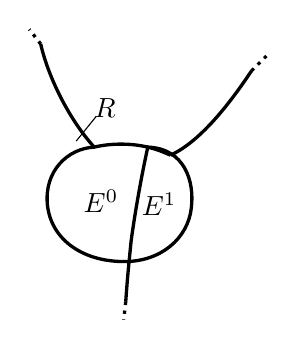
\begin{tikzpicture}[>=stealth,scale=0.85]
  \draw[very thick] (0.45,0.86) .. controls (1.0,0.84) and (1.15,0.35) .. (1.1,-0.05)
        .. controls (1.05,-0.5) and (0.65,-0.85) .. (0.1,-0.85)
        .. controls (-0.55,-0.85) and (-1.0,-0.5) .. (-1.05,0.0)
        .. controls (-1.1,0.5) and (-0.75,0.84) .. (-0.35,0.86)
        .. controls (-0.1,0.92) and (0.2,0.92) .. (0.45,0.86);%
  \draw[very thick] (0.79,0.74) .. controls (0.6,0.82) .. (0.45,0.86)
        .. controls (0.36,0.45) and (0.26,-0.1) .. (0.2,-0.55)
        .. controls (0.15,-1.05) .. (0.12,-1.45);
  \draw[very thick,dotted] (0.12,-1.45) -- (0.09,-1.72);%
  \draw[very thick] (0.79,0.74) .. controls (1.25,0.95) and (1.7,1.55) .. (2.0,2.0);
  \draw[very thick,dotted] (2.0,2.0) -- (2.25,2.25);
  \draw[very thick] (-0.35,0.86) .. controls (-0.75,1.3) and (-1.05,1.95) .. (-1.15,2.4);
  \draw[very thick,dotted] (-1.15,2.4) -- (-1.32,2.62);
  \node at (-0.19,1.45) {$R$};
  \draw (-0.32,1.32) -- (-0.62,0.95);%
  \node at (-0.25,0.05) {$E^{0}$};
  \node at (0.62,0.0) {$E^{1}$};
\end{tikzpicture}

图 3.6
\end{minipage}

由于 $\gamma(0)$ 与 $\gamma(1)$ 属于 $E\backslash R$ 的不同\trConnectedComponent，我们便得出：%
对某个 $0<t_{0}<1$ 有 $\gamma(t_{0})\in R$，从而 $f\bigl(\gamma(t_{0})\bigr)\geq\alpha$，%
于是
\[
\alpha\leq c(f,\mathcal{F})<\infty.
\]
鉴于\trMinimax{}引理，只须验证 $\mathcal{F}$ 在 $-\nabla f$ 的\trFlow{} $\varphi^{t}$ 下%
是正\trInvariant{}的。为此，只须证明：若 $x\in E^{j}_{\alpha}$，则对一切 $t\geq0$%
也有 $\varphi^{t}(x)\in E^{j}_{\alpha}$。而这由如下事实立即可得：对一切 $t\geq0$ 有%
$f\bigl(\varphi^{t}(x)\bigr)\leq f\bigl(\varphi^{0}(x)\bigr)=f(x)<\alpha$。
\end{proof}

关于\trMountainPassLemma{}的其他版本以及许多应用，我们请读者参阅 M.~\trStruwe{}的%
\emph{Variational methods} [208] 与 P.~\trRabinowitz{}的%
\emph{Minimax methods in critical point theory %
with applications to differential equations} [182] 两书。应当指出，若 $f$ 既不%
\trBoundedAbove{}也不\trBoundedBelow，那么要分析 $f$ 的定性行为、并找到满足上述%
\trEstimate{}（iv）的恰当的族 $\mathcal{F}$，往往是一件微妙的工作。对于我们的特殊%
\trFunctional{} $\Phi$，这将在下面两节中完成。不过，我们首先还须定义恰当的泛函分析框架。

至于\trCriticalPoint{}理论中更为精深的经典技巧，我们愿意提及 R.S.~\trPalais{}的%
经典论文 [173]（1970），以及 P.~\trBlanchard{}、E.~\trBruning{}的专著 [28]（1992）、%
J.~\trMawhin{}、M.~\trWillem{}的专著 [152]（1989），还有晚近的\trChang{} [39]（1993）。%
为\trCompact\trSymplecticManifold{}的\trLoopSpace{}上的\textbf{\trActionFunctional}（action functional）而设计的%
新方法将在第 6 章中描述。
